\documentclass[11pt,a4paper]{article}
% ============================================================
% Shared preamble for Claude Experiments reports (pdflatex)
% Include this AFTER \documentclass in each report:
%   \documentclass[11pt,a4paper]{article}
%   % ============================================================
% Shared preamble for Claude Experiments reports (pdflatex)
% Include this AFTER \documentclass in each report:
%   \documentclass[11pt,a4paper]{article}
%   % ============================================================
% Shared preamble for Claude Experiments reports (pdflatex)
% Include this AFTER \documentclass in each report:
%   \documentclass[11pt,a4paper]{article}
%   \input{../preamble}
% ============================================================
\usepackage[T1]{fontenc}
\usepackage[utf8]{inputenc}
\usepackage[english]{babel}
\usepackage[a4paper,top=2.5cm,bottom=2.5cm,left=2.5cm,right=2.5cm]{geometry}
\usepackage{amsmath,amssymb}
\usepackage{graphicx}
\usepackage{subcaption}
\usepackage{booktabs}
\usepackage{xcolor}
\usepackage[colorlinks=true,allcolors=blue]{hyperref}
\usepackage{microtype}
\usepackage{float}
\usepackage{array}
\microtypesetup{expansion=false}

% Color scheme
\definecolor{colMicro}{HTML}{222222}
\definecolor{colExact}{HTML}{2878b5}
\definecolor{colPlacement}{HTML}{e07a1f}
\definecolor{colBoundary}{HTML}{429c74}
\definecolor{colCurrent}{HTML}{c23b55}
\definecolor{colMM}{HTML}{c23b55}

\providecommand{\SIG}{\textcolor{green!50!black}{\textbf{*}}}
\providecommand{\NS}{\textcolor{gray}{n.s.}}
\providecommand{\DRMS}{\Delta\mathrm{RMST}}
\providecommand{\ci}[2]{$[{#1},\;{#2}]$}

% ============================================================
\usepackage[T1]{fontenc}
\usepackage[utf8]{inputenc}
\usepackage[english]{babel}
\usepackage[a4paper,top=2.5cm,bottom=2.5cm,left=2.5cm,right=2.5cm]{geometry}
\usepackage{amsmath,amssymb}
\usepackage{graphicx}
\usepackage{subcaption}
\usepackage{booktabs}
\usepackage{xcolor}
\usepackage[colorlinks=true,allcolors=blue]{hyperref}
\usepackage{microtype}
\usepackage{float}
\usepackage{array}
\microtypesetup{expansion=false}

% Color scheme
\definecolor{colMicro}{HTML}{222222}
\definecolor{colExact}{HTML}{2878b5}
\definecolor{colPlacement}{HTML}{e07a1f}
\definecolor{colBoundary}{HTML}{429c74}
\definecolor{colCurrent}{HTML}{c23b55}
\definecolor{colMM}{HTML}{c23b55}

\providecommand{\SIG}{\textcolor{green!50!black}{\textbf{*}}}
\providecommand{\NS}{\textcolor{gray}{n.s.}}
\providecommand{\DRMS}{\Delta\mathrm{RMST}}
\providecommand{\ci}[2]{$[{#1},\;{#2}]$}

% ============================================================
\usepackage[T1]{fontenc}
\usepackage[utf8]{inputenc}
\usepackage[english]{babel}
\usepackage[a4paper,top=2.5cm,bottom=2.5cm,left=2.5cm,right=2.5cm]{geometry}
\usepackage{amsmath,amssymb}
\usepackage{graphicx}
\usepackage{subcaption}
\usepackage{booktabs}
\usepackage{xcolor}
\usepackage[colorlinks=true,allcolors=blue]{hyperref}
\usepackage{microtype}
\usepackage{float}
\usepackage{array}
\microtypesetup{expansion=false}

% Color scheme
\definecolor{colMicro}{HTML}{222222}
\definecolor{colExact}{HTML}{2878b5}
\definecolor{colPlacement}{HTML}{e07a1f}
\definecolor{colBoundary}{HTML}{429c74}
\definecolor{colCurrent}{HTML}{c23b55}
\definecolor{colMM}{HTML}{c23b55}

\providecommand{\SIG}{\textcolor{green!50!black}{\textbf{*}}}
\providecommand{\NS}{\textcolor{gray}{n.s.}}
\providecommand{\DRMS}{\Delta\mathrm{RMST}}
\providecommand{\ci}[2]{$[{#1},\;{#2}]$}

\title{CE-07: Calibration Floor\\Development Report --- Pilot Results}
\author{Two-Layer CTMC Experiments Pipeline}
\date{August 4, 2026}
\begin{document}\maketitle
\begin{abstract}
CE-07 asks how much MicroMacro error can be removed by a scalar rescaling of $\beta_{out}$ and how much remains structural. In nine pilot cells with 40 paired replications, the selected scale improved absolute normalized RMST error in every cell, but a substantial residual remained. The selected factor varied from 0.5 to 1.2, so no universal calibration constant is supported. These are development results because selection and evaluation use the same replications and the full grid is still pending.
\end{abstract}
\section{Design}
The pilot varied $r\in\{0.5,1,2\}$ and $d\in\{4,6,12\}$ at $k=5$. For each cell, Full Micro was run once per paired replication and MicroMacro was evaluated over a discrete calibration grid. The reported $c^*$ minimizes terminal mean mismatch on the same 40 replications. The structural fraction is $|\Delta\mathrm{RMST}_{cal}|/|\Delta\mathrm{RMST}_{uncal}|$.

\section{Results}
\begin{table}[H]\centering
\caption{Pilot averages over degree values.}
\begin{tabular}{rrrrr}\toprule
$r$ & Mean $c^*$ & Uncalibrated norm. error & Calibrated norm. error & Structural fraction\\\midrule
0.5 & 0.917 & -0.0315 & -0.0117 & 0.431\\
1.0 & 0.567 & -0.1375 & -0.0498 & 0.373\\
2.0 & 0.500 & -0.3339 & -0.2408 & 0.712\\
\bottomrule\end{tabular}
\end{table}
Calibration reduced absolute normalized error in all 9 cells. Nevertheless, cell-level structural fractions span approximately 0.22--0.78. At high export ratio, scalar rate reduction removes only a minority of the error. The selected $c^*$ also depends on both $r$ and $d$, and reaches the lower candidate bound in several cells.

\begin{figure}[H]\centering
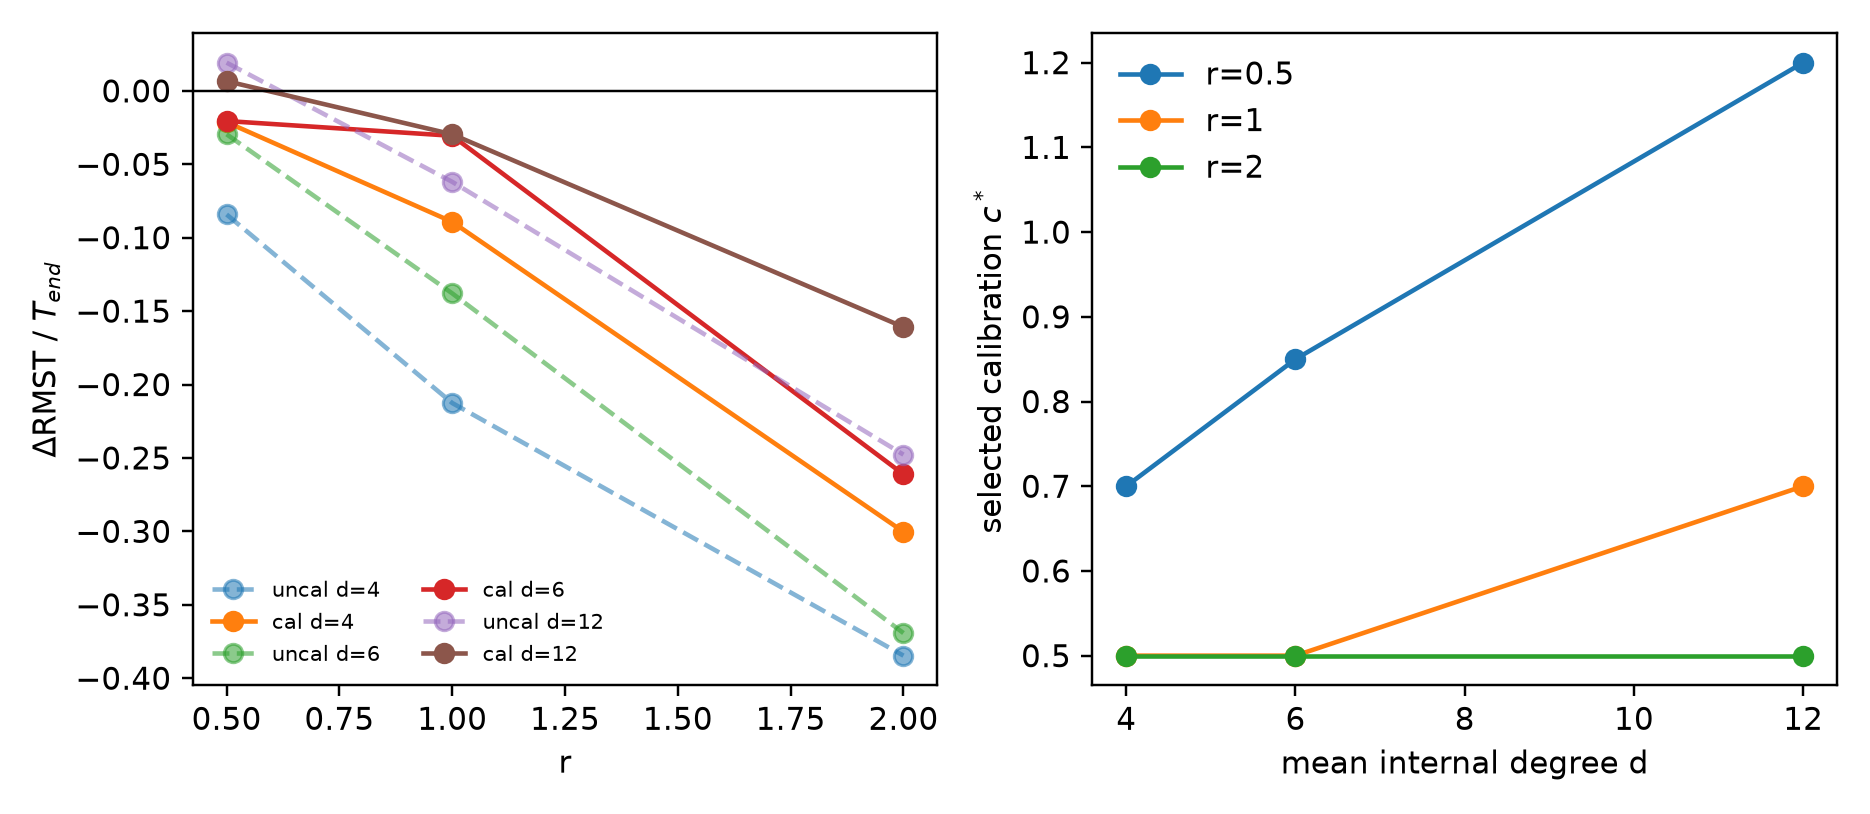
\includegraphics[width=.9\linewidth]{figures/calibration_floor.png}
\caption{In-sample calibration effect (left) and selected scale (right). Each point uses 40 paired replications.}
\end{figure}

\section{Implications}
A global $\beta_{macro}$ multiplier is useful as a baseline calibration layer, not as a complete correction. The remaining error is consistent with state-dependent gateway reachability and import timing that a constant cannot represent. The dependence of $c^*$ on $r$ and $d$ supports a parameters-only adaptive correction, but choosing a flexible function from these same cells would overfit.

The full run should separate fitting from evaluation: select $c$ on a training seed block or nested bootstrap, then report held-out RMST and completion. Until that is done, these values estimate an optimistic calibration floor and must not be used as final performance claims.

\section*{Status and reproduction}
\textbf{DEVELOPMENT RESULTS --- NOT FINAL.} Full CE-07 is queued after the currently running ER-01 pilot.\\
\texttt{.venv/bin/python extrascripts/run\_ce07\_calibration\_floor.py --grid full --workers 12 --resume}
\end{document}
